%% Set nonacm to remove copyright, conf info, etc
\documentclass[sigconf, nonacm]{acmart}
%\documentclass{article}

\usepackage{amsmath}
\usepackage{algorithm} 
\usepackage{algpseudocode}
\usepackage{listings}
\usepackage{float}
\usepackage{placeins}
%\restylefloat{table*}
\lstset{language=C++,
        basicstyle=\ttfamily,
        keywordstyle=\color{blue}\ttfamily,
        stringstyle=\color{red}\ttfamily,
        commentstyle=\color{green}\ttfamily,
        morecomment=[l][\color{magenta}]{\#},
        xleftmargin=.1\linewidth,
        xrightmargin=.1\linewidth
}

\begin{document}

\title{Procedural Rendering with Ray Marching}

\author{Christian A. Robles}
\affiliation{%
  \institution{University of Southern California}
  \city{Los Angeles}
  \country{USA}}
\email{roblesch@usc.edu}

\author{Hoseung Lee}
\affiliation{%
  \institution{University of Southern California}
  \city{Los Angeles}
  \country{USA}}
\email{hoseungl@usc.edu}

\author{Samuel Yin}
\affiliation{%
  \institution{University of Southern California}
  \city{Los Angeles}
  \country{USA}}
\email{slyin@usc.edu}

\author{Vansh Dhar}
\affiliation{%
  \institution{University of Southern California}
  \city{Los Angeles}
  \country{USA}}
\email{vdhar@usc.edu}

%% Replace default author header with empty
\renewcommand{\shortauthors}{}

%%
%% The abstract is a short summary of the work to be presented in the
%% article.
\begin{abstract}
Ray tracing requires evaluation of explicit ray-surface intersections. Complex shapes can be difficult to model as they must be broken down into an aggregate of many primitives, and ray tracing scales poorly with the number of objects in the scene. Ray marching allows us to model complex shapes more efficiently by implicitly identifying intersections with surfaces through the use of a Signed Distance Function. With ray marching, we can efficiently model and render complex shapes, create new shapes with constructive solid geometry, and render procedural materials and surfaces.
\end{abstract}

%% A "teaser" image appears between the author and affiliation
%% information and the body of the document, and typically spans the
%% page.
\begin{teaserfigure}
  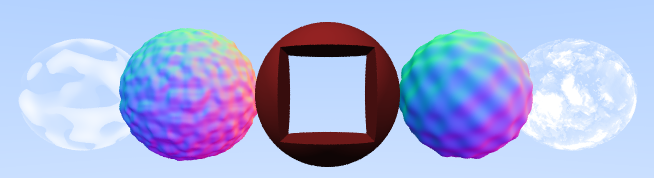
\includegraphics[width=\textwidth]{images/teaser.png}
  \caption{Procedural Perturbations, Constructive Solid Geometry, Marched Depth Clouds}
  \Description{A sample of procedural surfaces and materials produced by ray marching.}
  \label{fig:teaser}
\end{teaserfigure}

%%
%% This command processes the author and affiliation and title
%% information and builds the first part of the formatted document.
\maketitle

\section{Introduction}

Let a scene consist of a set of surfaces in a 3d world coordinate space with a camera at some position. We will generate an image by sending rays through each pixel coordinate in the camera's viewport, determining if an intersection occurs, and evaluating a material at that intersection.

Consider a ray tracing renderer. We determine the color of each pixel by comparing this ray to each object in the scene and determining if an intersection occurs, then evaluating material properties. Consider a simple sphere primitive. Ray-sphere intersection requires solving $|(P(t)-C)|^2 = r^2$ for some ray $P(t) = A + tb$ and some sphere with center $C$ and radius $r$. We must additionally decide which intersection point is nearest and in front of the camera, if we are viewing from the inside or outside of the sphere, and calculate a surface normal to calculate the appropriate material color at that intersection. Even for a relatively simple primitive such as a sphere, determining a ray-surface intersection for every surface in a scene is a computationally expensive task.

\begin{figure}[h]
  \centering
  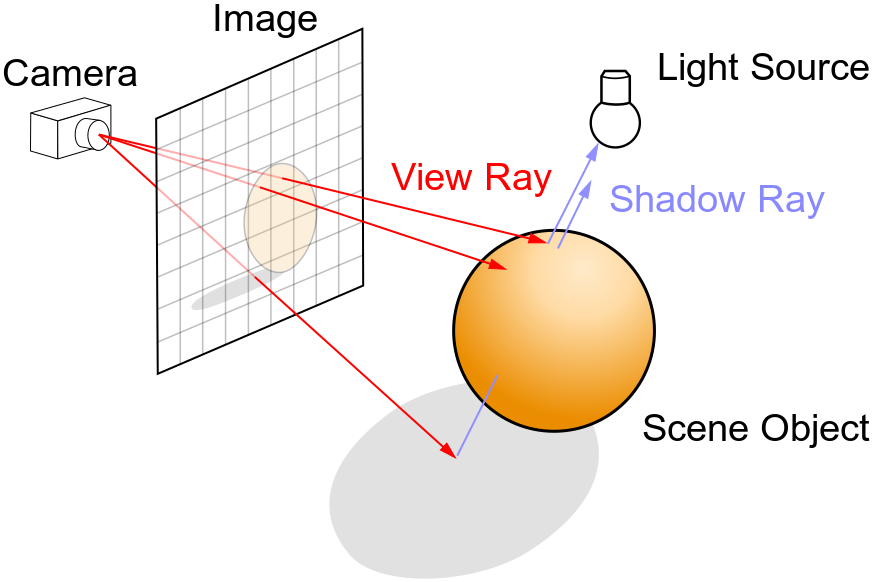
\includegraphics[width=0.6\linewidth]{images/Ray_trace_diagram.png}
  \caption{Evaluating a scene with ray tracing, via Wikimedia
    Commons. (\url{https://w.wiki/55Pu}).}
\end{figure}

In ray tracing, we are limited to only those surface primitives where we can explicitly calculate a ray-surface intersection. Planar surfaces can be solved with a ray-plane intersection and inside-outside test. Various shapes and orientations of surfaces can be derived by model transformations of translations rotations and scales. Higher complexity surfaces that would be otherwise too difficult to evaluate directly can be modeled by the composition of many planar primitives, but performance scales poorly with the number of surfaces in the scene. Complex materials additionally require even more rays to be cast for lighting, scattering, and transmission. Effects like soft shadows and anti-aliasing further degrade performance, requiring a polynomial total number of rays to be cast to determine the color of an individual pixel.

Consider a ray marching renderer. We again determine the color of each pixel by evaluating the scene in the direction of a camera ray. Rather than evaluating the intersection between this ray and any surface in the scene, we instead let the scene provide a \textit{Signed Distance Function} which evaluates some point $p(x,y,z)$ and returns the approximate distance $d$ between $p$ and the nearest surface in the scene. If the value is positive, we are $d$ units away from the nearest surface. If it is negative, we are $d$ units inside the surface. If $d$ is close to zero, then we can say we are intersecting the nearest surface. Starting from $t = 0$, we will for each ray evaluate the distance to the closest surface in the scene $d$ and march $d$ units in the direction of the ray. We will evaluate the scene again and repeat this process until $d$ is near-zero, or until the ray terminates due to a march limit or a maximum depth along the ray $t_{max}$.

\begin{figure}[h]
  \centering
  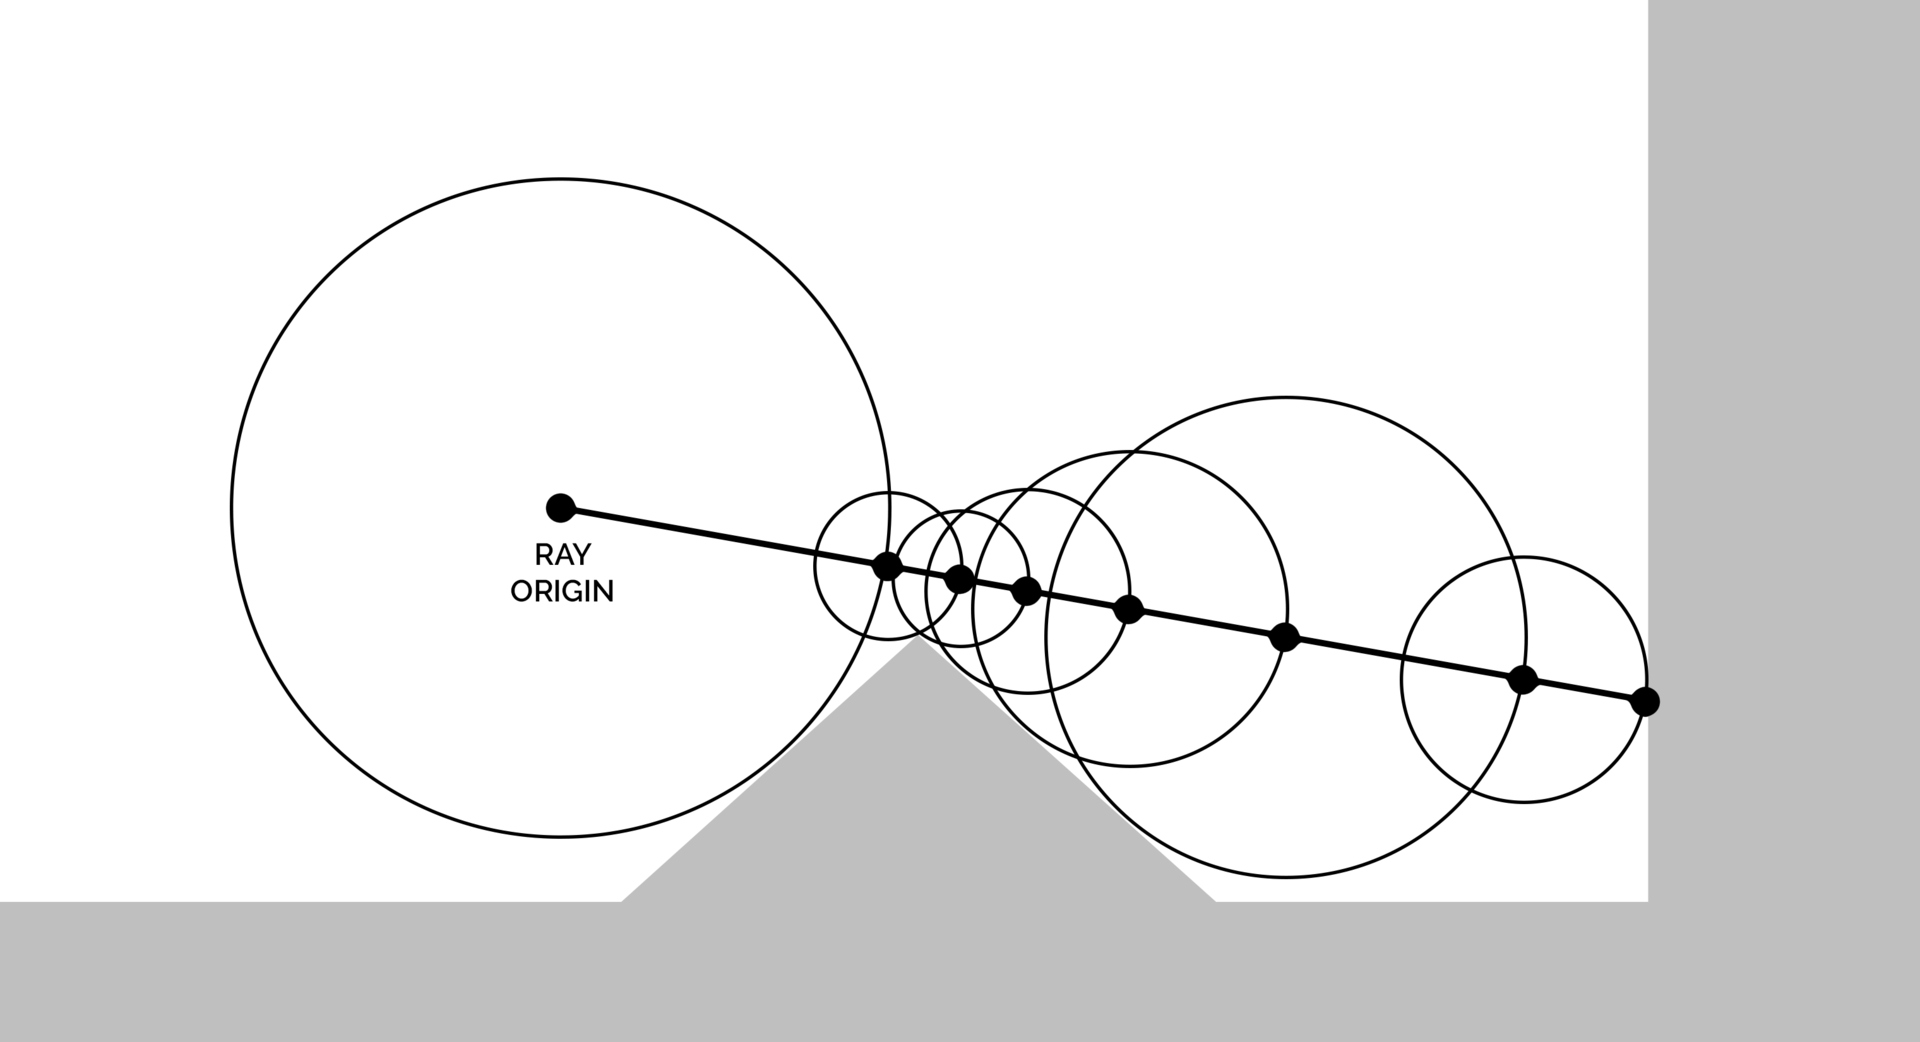
\includegraphics[width=0.6\linewidth]{images/Visualization_of_SDF.png}
  \caption{Marching along a ray using the SDF of the scene, via Wikimedia
    Commons. (\url{https://w.wiki/55Ps}).}
\end{figure}

In the ray marching model, ray-surface intersections no longer require explicit evaluation of intersection formulae. Instead, we implicitly model ray-surface intersections by marching down the ray until the distance to the scene is near-zero. With these implicit intersections, we are no longer constrained to simple surface primitives. We can render any surface that has a defined distance function. Additionally, we can model scenes of complex functions like fractals or noise functions by mapping their values to distance values. We can combine distance functions for multiple surface primitives by union or intersection, and interpolate between them with smoothing functions. We can model 3D materials by stepping through them and evaluating functions along each step. Surface normals no longer require explicit evaluation and can instead be calculated by the gradient of the distance function.

\section{Renderer Implementation}

We implement our renderer from reference code provided by Peter Shirley's \textit{Ray Tracing in One Weekend}. We use the template code Peter provides up to Chapter 4: \textit{Rays, a Simple Camera, and Background}. We also use the Anti Aliasing techniques from Chapter 7, and the Positionable Camera from Chapter 11. We follow Peter's interface patterns for surfaces and materials, with some modifications. We rename \textit{hittable} to \textit{surface}, and \textit{hittable\_list} to \textit{scene}. We discard all ray tracing functionality and replace it with our implementations of ray marching.

\subsection{Interfaces}

\subsubsection{Surface}

The \textit{surface} class is an interface for intersectable objects in the scene. Any class that implements \textit{surface} must accept in its constructor a valid pointer to a \textit{material}. It must provide an implementation for

\begin{lstlisting}
double distance(const vec3& p)
\end{lstlisting}

The \textit{distance} function returns the signed distance from some point $p(x,y,z)$ and the surface. If the result is negative, $p$ is considered inside the surface. 

\subsubsection{Material}

A class that implements the \textit{material} interface must implement

\begin{lstlisting}
vec3 color(ray &r, vec3 p, vec3 N,
           vector<light> lights)
\end{lstlisting}

The \textit{color} function accepts an incoming ray, an intersection point, a surface normal, and a list of directional lights. It returns the color of the material evaluated by those parameters.

\subsubsection{Scene}

The \textit{scene} class manages objects and lights in a scene, and maintains internal lists of pointers to instances of these classes. It provides the following key functions:

\begin{lstlisting}
bool near_zero(double d)
\end{lstlisting}

Returns \textit{true} if $d$ is smaller than machine-epsilon: the difference between 1.0 and the next value representable by the floating-point type.

\begin{lstlisting}
double distance_estimator(vec3 p)
\end{lstlisting}

Iterates over the list of scene surfaces and returns the distance from some point $p(x,y,z)$ and the surface nearest that point.

\begin{lstlisting}
vec3 normal(vec3 &p)
\end{lstlisting}

Returns the "surface normal" at some point $p(x,y,z)$. We take a small step along each of the $x, y, z$ axes and return the unit length vector in the direction of the gradient of the distance function.

\begin{lstlisting}
bool march(ray& r, hit_record& rec)
\end{lstlisting}

Beginning at $t = 0$, \textit{march} evaluates the distance from the point along the ray $r$ at $t$ to the nearest surface in the scene. If the distance is near zero, \textit{march} will terminate and return true, and store the information about the intersection and the material of the surface intersected on the hit record. If the distance is not near zero, it will increase $t$ by $d$ with a minimum step size of $0.001$ and evaluate the distance estimator again. Will terminate if a surface is hit or if $t \geq t_{max}$.

\begin{lstlisting}
vec3 ray_color(ray& r)
\end{lstlisting}

Evaluates a ray by performing marching. If a surface is hit, queries the material properties for the color evaluated at the point of intersection. Otherwise, returns the background color of the scene.

\subsection{Surface Primitives}

The following classes provide implementations for \textit{surface}. In each formulation, $p$ refers to some point $p(x,y,z)$ along a ray. In our notation $||v||$ denotes the Euclidean norm for some vector $v$, and $|v|$ denotes a component-wise absolute value for some vector $v$. $Min$ and $Max$ operations are also component-wise.

\subsubsection{Sphere}

An instance of \textit{sphere} is specified by a center $C$ and a radius $r$.
$$
distance = ||(p - C)|| - r
$$

\subsubsection{Box}

An instance of \textit{box} is specified by a vector $B$ representing the distance from the center to the edges of the box -
\begin{gather*}
q = |p| - B\\
distance = ||max(q,0)|| + min(max(q_x,max(q_y,q_z)),0)
\end{gather*}

\subsubsection{Equilateral Triangular Prism}

An instance of a triangular prism is specified by a center C, prism length L, and triangle height H.
\begin{gather*}
q = |p - C| \\
distance = max(q_z-H_y,max(q_x*0.866+p_y/2,-p_y)-H_x/2)
\end{gather*}

\subsubsection{Cylinder}

An instance of a cylinder is specified by a center $C$, height $H$, and radius $r$.
\begin{gather*}
q = p - C\\
d_x = |length(q_{xz}) - r|\\
d_y = |length(q_y) - H|\\
distance = min(max(d_x, d_y), 0) + ||max(d,0)||
\end{gather*}

\subsubsection{Pyramid}

An instance of a pyramid with a constant square $1\times1$ base is specified by a center $C$ and height $H$.
\begin{gather*}
a = H^2 + 1/4\\
p = p - C\\
p_{xz} = |p_{xz}|\\
p_z > p_x\ ?\ p_{xz} = p_{zx}\\
p_{xz} = p_{xz} - 1/2\\
b = (p_z, H*p_y - p_x/2, H*p_x + p_y/2)\\
c = max(-b_x,0)\\
d = clamp((b_y-p_z/2)/(a+1/4), 0, 1)\\
e = a*(b_x+s)^2 + b_y^2\\
f = a*(b_x+d/2)^2 +(b_y-a*d)^2\\
min(q_y,-q_x*a-q_y/2) > 0\ ?\ g = 0 : g = min(a,b)\\
distance = \sqrt{(g+b_z^2)/a} * sign(max(b_z,-p_y))
\end{gather*}

\subsubsection{Infinite Cylinder}
An instance of an infinite cylinder is specified by a center $C$ and radius $R$. Its distance function is identical to a cylinder without comparing the $y$ coordinate.

\begin{figure}[h]
  \centering
  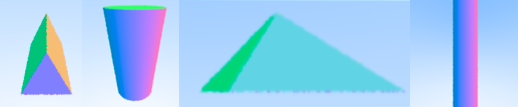
\includegraphics[width=\linewidth]{images/surface-primitives.png}
  \caption{Triangular Prism, Cylinder, Pyramid, Infinite Cylinder}
\end{figure}

\subsection{Materials}
\subsubsection{Diffuse}
The \textit{diffuse} class implements the \textit{color} function to return the color $C$ as
$$
    C = (Ks\sum_L(le(R\cdot E)^s]) + (Kd\sum_L (le(N\cdot L)) + (Ka*la)
$$

\subsubsection{Clouds}

We implement the materials perlin\_cloud\_2d, perlin\_cloud\_3d, gardner\_cloud\_2d and gardner\_cloud\_3d by mapping surface coordinates to a noise function and attenuating output color by march depth. Described in section 4.

\subsubsection{Normals}

Maps a normal $N$ to RGB as
$$
    C = (N + 1)/2
$$

\subsubsection{Flat}

Returns a constant color.

\section{Constructive Solid Geometry}
Constructive Solid Geometry is the technique of combining primitives to form a more complex object using Boolean operators such as \textit{union}, \textit{difference}, and \textit{intersection}. Ray marching makes CSG easy. When a signed distance function returns a positive value, it means it is outside of the object. A negative SDF means we are inside of the object. When can use this property to implement the Boolean operations with combination and negation of the SDFs for two or more surfaces.

\subsubsection{Union}
The union of two objects is computed simply by the minimum of the distances of two objects. Since we are already returning the surface nearest to the point in our distance estimator function, this operation is already handled by the ray marching algorithm.

\subsubsection{Intersection}
The intersection of two objects is the area in which both objects converge. To get the intersection of two objects, distance to both objects should be less than or equal to zero. This creates an object that only exists at the intersection of the two objects.

\subsubsection{Difference}
Finally, the difference of two objects is the maximum of the distance functions with one function negated. Flipping the sign inverts the object so everything that was considered inside an object is now outside and vice versa. The object now only exists if it is inside the non-inverted object and outside of the inverted object, resulting in one area "cutting" into the other. 

\begin{figure}
  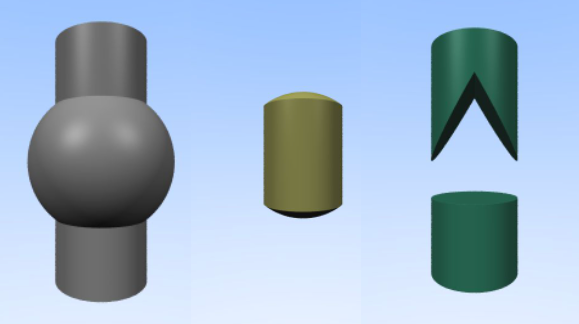
\includegraphics[width=0.75\linewidth]{images/union-intersection-difference.png}
  \caption{Union, Intersection, Difference}
\end{figure}

\subsubsection{Smoothing}
We can blend the intersection of two objects by interpolating where the objects approach each other. We can apply smoothing to union as

\begin{lstlisting}
h = max(k - abs(d1 - d2), 0.0);
return min(d1, d2) - h * h * 0.25/k;
\end{lstlisting}

Where $k$ is some value between 0 and 1 and controls the amount of smoothing. For intersection and difference, we apply the same logic as before: using max instead of min and flipping the sign for the difference.

\begin{figure}
  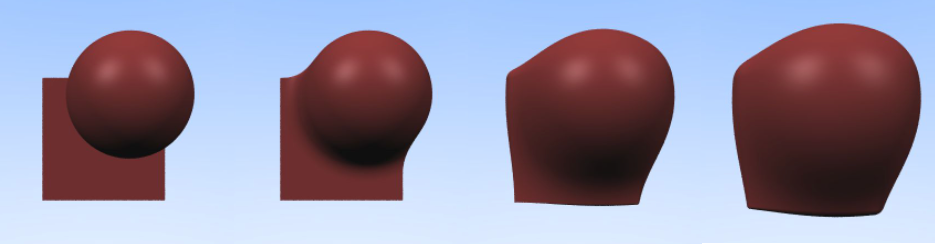
\includegraphics[width=\linewidth]{images/smoothing.png}
  \caption{Smooth union with k = 0, 0.2, 0.6, 0.9}
\end{figure}

\section{Procedural Textures}

Procedural generation of 3D clouds is a complex challenge in rendering. Clouds in real-time applications are often drawn by mapping pre-rendered 2D textures at distances or on volumes not interactable by the camera. However, these approaches fall apart when viewed at shallow angles or positioned near the camera. We will examine how ray marching can be leveraged to generate 3D textures on marchable depth surfaces to approximate the appearance of clouds.

We will examine two noise functions for generating cloud textures. The first is proposed by Geoffrey Y. Gardner in his paper \textit{Visual Simulation of Clouds}. The second is the famous Perlin Noise, originally proposed by Ken Perlin in his paper \textit{An image synthesizer}.

\subsection{Gardner Noise}

In \textit{Visual Simulation of Clouds}, Gardner proposes a texturing function that approximates the appearance of clouds. We refer to this function as \textit{Gardner Noise}. It models textures as a product of sums of $3<n<8$ sine waves
\begin{align*}
    T(X,Y,Z)=&k\sum_{i+1}^n[C_i\sin (FX_ix+PX_i)+T_0]\\
    &\times\sum_{i=1}^n[C_i\sin (FY_iY+PY_i)+T_0]
\end{align*}

Where frequencies and coefficients are chosen by
\begin{align*}
    FX_{i + 1} &= 2FX_i \\
    FY_{i + 1} &= 2FY_i \\
    C_{i + 1} &= .707C_i
\end{align*}

And $PX_i$ and $PY_i$ are determined by
\begin{align*}
    PX_i&=\pi /2\sin (.5FY_{i-1}Y)+\pi \sin(FX_iZ/2)&for\ i > 1\\
    PY_i&=\pi /2\sin (.5FX_{i-1}iX)+\pi \sin(FX_iZ/2)&for\ i >1
\end{align*}

$T_0$ is a parameter controlling contrast, and $k$ is computed such that the maximum of $T(X,Y,Z)\approx1$.

\subsection{Perlin Noise}

In his paper \textit{An image synthesizer}, Ken Perlin describes a noise function that accepts a $n$-vector and returns a value with the qualities of statistical invariance under rotation and translation and a narrow bandpass limit in frequency. We use $3$-noise, which is constructed by

1. Construct a 3 dimensional grid of size $x$ by $y$ by $z$.

2. Assign to each grid intersection a pseudo-random unit length gradient vector $v_{x_i,y_i}(x,y,z)$

3. For some input $p(x,y,z)$, determine which grid cell contains $p$. Identify the corners of that cell and calculate an offset vector from each corner to $p$.

4. For each corner, calculate the dot product of its offset vector and its gradient vector.

5. Interpolate the grid corner dot products at $p$ and return this value as the result.

\subsection{Procedural Clouds}

Using noise to generate textures is simple. We evaluate a ray-surface intersection and pass the point $p(x,y,z)$ to one of these functions and use the $[0, 1.0]$ result as a texture value $T$. Gardner phase and coefficient parameters can be tuned to modify the size and variance of the cloud-like textures, and Perlin noise can be tuned to map input coordinates to larger or smaller gradient grids for fuzzier or granular textures.

We can additionally march through surfaces to generate more convincing 3D textures. We accept as a material parameter the approximate depth of a surface and use this value to determine a marching step bound and step size. We use a cutoff threshold to march past low texture values and attenuate the final result by a combination of step size and step count.

\begin{figure}[h]
  \centering
  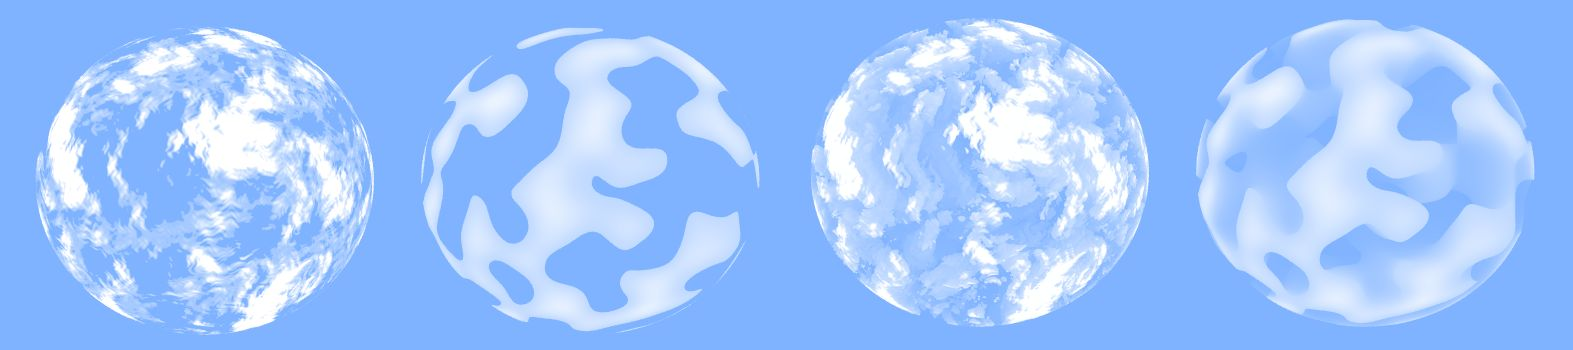
\includegraphics[width=\linewidth]{images/procedural_clouds.jpg}
  \caption{Surface Mapped and Depth Marched Gardner \& Perlin Clouds}
\end{figure}

\section{Procedural Surfaces}

In section 3 we saw how we can alter surfaces by altering the SDF. We can create a new class of surfaces we call procedural surfaces by combining this technique with our noise functions.

Procedural surfaces are analogous to the bump mapped textures. Bump maps use lighting effects to provide the appearance of surface variation, but do not actually affect surface geometry. With procedural surfaces, we can create more convincing effects by altering the surface directly. Additionally, we can render fractals and other complex functions by mapping values to an SDF over some defined set of inputs.

\subsection{Displacement Surfaces}

Sphere perturbations are simple - for some displacement function $D$, we add its value to the SDF of a sphere
$$
distance = (p - C) - r + D
$$

We implement two displacement surfaces. \textit{Perlin Sphere} uses Perlin Noise (4.1.2) to evaluate $D(x,y,z)$. \textit{Perturbed Sphere} implements $D$ as a sum of sine waves
$$
D(x,y,z) = c*\sin(\varphi + x)*\sin(\varphi + y)*\sin(\varphi + z)
$$

Where $c$ is some coefficient that modulates the intensity of displacement and $\varphi$ is some constant phase shift.

\begin{figure}[h]
  \centering
  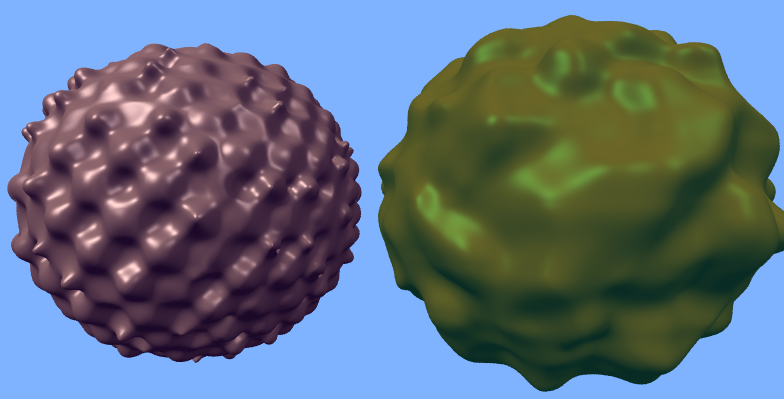
\includegraphics[width=.75\linewidth]{images/perturbed-spheres.png}
  \caption{Diffuse Perturbed and Perlin Spheres}
\end{figure}

\subsection{Fractals}

Fractals are infinitely complex mathematical shapes that recurse as you zoom into an area of a fractal. These infinitely complex fractals could not be rendered in ray tracing due to having no analytical intersection. With ray marching, we can use distance functions to render visualizations of complex relations such as the Mandelbulb fractal. Our implementation of a Mandelbulb is formulated as
\begin{gather*}
r={\sqrt {x^{2}+y^{2}+z^{2}}}\\
\phi=\arctan{\frac{y}{x}}=\arg(x+y_i)\\
\theta=\arctan{\frac{\sqrt{x^{2}+y^{2}}}{z}}=\arccos{\frac{z}{r}}\\
\mathbf{v} ^{n}:=r^{n}{\big \langle }\sin {\big (}f(\theta ,\phi ){\big )}\cos {\big (}g(\theta ,\phi ){\big )},\sin {\big (}f(\theta ,\phi ){\big )}\\
\sin {\big (}g(\theta ,\phi ){\big )},\cos {\big (}f(\theta ,\phi ){\big )}{\big \rangle }
\end{gather*}

\begin{figure}[h]
  \centering
  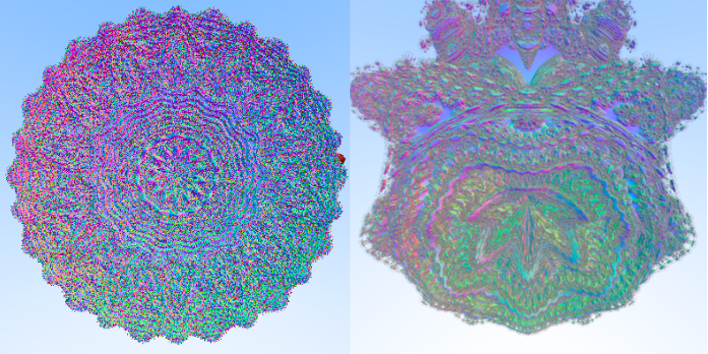
\includegraphics[width=0.75\linewidth]{images/fractals.png}
  \caption{Mandelbulbs at different view angles}
\end{figure}

For complex shapes, it is important to supersample rays to reduce aliasing artifacts introduced by high variance within pixel coordinates.

\section{Parallelization}

\begin{table*}[!htbp]
\begin{center}
    \begin{tabular}{ | l | l | l | l | l | l | l | l |}
    \hline
    \textbf{Resolution}  & \textbf{Block Size} & \textbf{Number of Samples} & \textbf{Parallel Time} & \textbf{Serial Time}  & \textbf{Speed Up} & \textbf{Branch Efficiency} & \textbf{A/T Occupancy} \\ \hline
    256x256	& 8x8	& 8	& 0.027s	& 29.483s &	1091.963	& 99.27	& 83.42/87.5  \\ \hline
    256x256	& 16x16	& 8	& 0.031s & 29.483s &	951.065	& 99.27	& 80.14/87.5  \\ \hline
    256x256	& 32x8	& 8	& 0.042s	& 29.483s &	701.976	& 97.54 & 76.59/83.33  \\ \hline
    256x256	& 128x1	& 8	& 0.038s	& 29.483s &	775.868	& 99.27	& 77.37/83.33  \\ \hline
    256x256	& 256x1	& 8	& 0.033s	& 29.483s &	893.424	& 98.65	& 79.28/87.5 \\ \hline
    512x512	& 8x8	& 8	& 0.073s	& 117.817s &	1613.932	& 99.38	& 82.74/87.5  \\ \hline
    512x512	& 16x16	& 8	& 0.081s	& 117.817s &	1454.531	& 99.27	& 78.94/87.5  \\ \hline
    512x512	& 32x8	& 8	& 0.096s	& 117.817s &	1227.260	& 99.27	& 72.41/83.33  \\ \hline
    512x512	& 128x1	& 8	& 0.092s	& 117.817s &	1280.620	& 98.65	& 74.53/87.5 \\ \hline
    512x512	& 256x1	& 8	& 0.093s	& 117.817s &	1266.849	& 98.65	& 74.68/87.5 \\ \hline
    1024x1024	& 8x8	& 8	& 0.191s	& 476.936s &	2497.047	& 99.38	& 83.65/87.5  \\ \hline
    1024x1024	& 16x16	& 8	& 0.209s	& 476.936s &	2281.990	& 98.65	& 81.12/87.5  \\ \hline
    1024x1024	& 32x8	& 8	& 0.243s	& 476.936s &	1962.700	& 99.38	& 74.64/83.33  \\ \hline
    1024x1024	& 128x1	& 8	& 0.241s	& 476.936s &	1978.988	& 98.65	& 75.23/83.33  \\ \hline
    1024x1024	& 256x1	& 8	& 0.244s	& 476.936s &	1954.656	& 98.65	& 75.87/83.33  \\ \hline
    \end{tabular}
    \begin{center}
    \caption{In the above table, we list the different parameter configurations of our CUDA program and the SpeedUp achieved for those configurations. We also list the Branch Efficiency and Achieved/Theoretical Occupancy for each configuration. }
    \end{center}
\end{center}
\end{table*}

A ray marching rendering system requires more computational resources than ray tracing due to the simple fact that in ray tracing, computation is done only at the point of object intersection. In ray marching, distance functions are evaluated for every iteration of the march. Thus, to improve the execution time of our renderer, we utilize the power of parallel computing with the help of CUDA programming and NVIDIA GPU.

\subsection{Platform Used}
Hardware specification:
The CUDA program was tested on a 64-bit operating system with 16 GB of Ram and an AMD Ryzen 9 5900HX processor, along with a Nvidia GeForce RTX 3070 GPU (Laptop version).

Software Specification: The hardware ran on Windows 11 OS and we used Microsoft Visual Studio as our programming IDE to develop the CUDA program. We also used Nvidia Nsight Compute to profile our CUDA program to better understand the resource utilization of the GPU while the program was running.

\subsection{CUDA Programming Overview}

In GPU programming, there are several parameters on both the software side and the hardware side that affect performance. Whenever a part of the program is outsourced to a GPU to be computed, On the software side: the total number of threads/ processors used are represented by a "Grid", which in our case will represent the image being rendered, therefore, the total number of threads will be equal to the number of pixels in our image. These threads are further divided into blocks which are independent units of execution with no communication possible between different blocks. 

\begin{figure}[h]
  \centering
  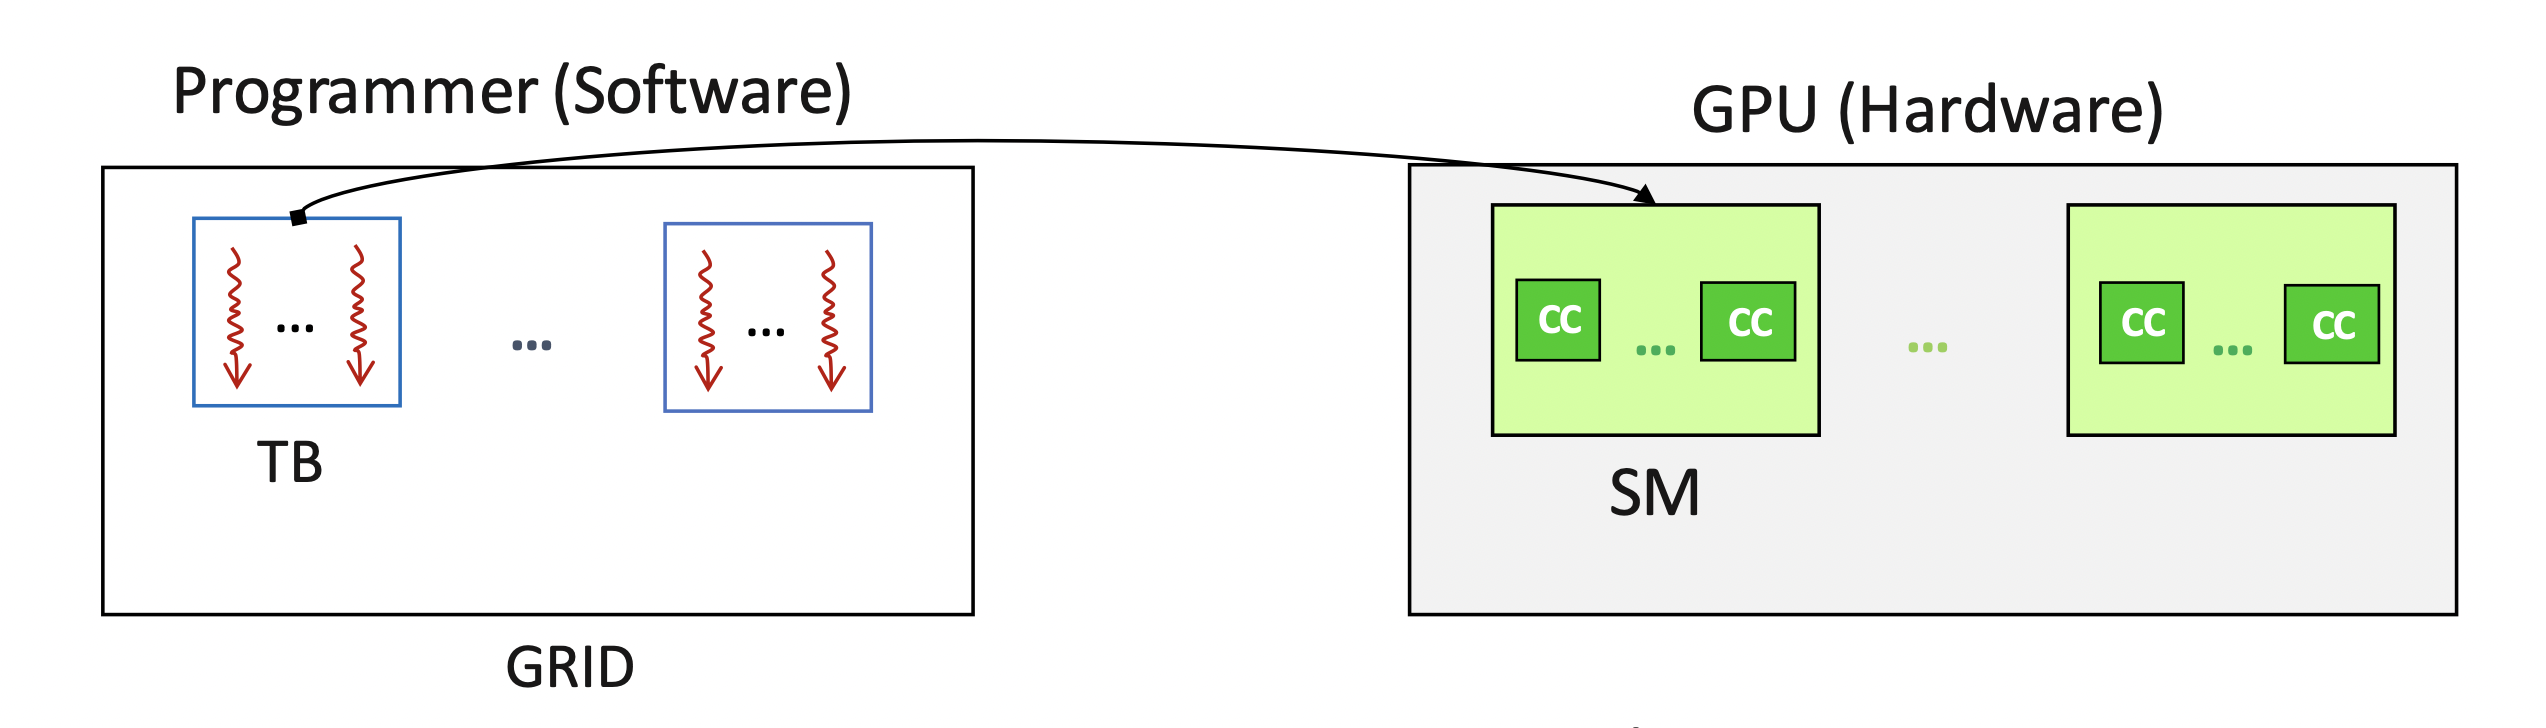
\includegraphics[width=1\linewidth]{images/GPU_description.png}
  \caption{Diagram depicting software and hardware abstraction for GPU programming}
\end{figure}

Now on the hardware side: The total number of cores/processors in the GPU are divided between Streaming Multiprocessors (SMs) such that each block can be executed only on a single SM with the possibility of several blocks being executed concurrently on the same SM if the hardware resource allows it. Thus, fine-tuning parameters like block size for an image of specific resolution being renderer based on the resource utilization of the hardware can lead to a significant increase in SpeedUp.

\begin{align}
    SpeedUp &= S/P
\end{align}
here, S: is the Program Serial Execution Time and P: is the Program Parallel Execution time

\subsection{Parallel Algorithm}
This section describes the algorithm/psuedo code run by each thread of the program.
\begin{algorithm}[H]
\caption{: Algorithm executed by each Thread/Pixel}\label{alg:cap}
\begin{algorithmic}
% \Require $n \geq 0$

\State $i \gets ThreadIdx.x$ + $ BlockDim.x * BlockIdx.x$
\State $j \gets ThreadIdx.y$ + $ BlockDim.y * BlockIdx.y$
\Ensure $i < Image\_Width $ and $ j < Image\_Height $
\State $N \gets No\_of\_Samples$
\State $Color_{ij} \gets 0$
\While{$N \neq 0$}
%\If{$N$ is even}
    \State $i += Random(-1,1)$
    \State $j += Random(-1,1)$
    \State $ray =  Compute\_Ray( Camera\_Info, i, j)$  
    \State $Color_{ij} +=  Compute\_Color( 3D\_Scene, ray)$ 
%\ElsIf{$N$ is odd}
    \State $N \gets N - 1$
%\EndIf
\EndWhile
\State $FrameBuffer[j,i] =  Color_{ij}/No\_of\_Samples$ 
\end{algorithmic}
\end{algorithm}

\subsection{Experiments and Results}

As discussed in section 6.2, several parameters can affect the execution time of our rendering system. The focus of our experiments will be to understand the range of the parameters for which we can achieve maximum speedup. The main parameters of focus will be: Block size (Number of Threads in each block), Grid size (Image Resolution). To better understand Resource utilization of our GPU based on these parameters we will also look at Branch Efficiency and Achieved Occupancy.

Branch Efficiency is the ratio of similar work done by threads in a block to the total work done by threads in a block. (Note: Threads in a block run concurrently only if they do similar work, thus, this ratio should be high to achieve maximum performance). Achieved Occupancy is the ratio of number of active processors to the total number of processors in a Streaming Multiprocessor. (Note: This ratio should be as close to theoretical occupancy as possible to achieve maximum performance).

Thus, for a range of parameter values the Program Parallel Execution Time, Program Serial Execution Time and SpeedUp can be seen in Table 1. By analysing the results in Table 1, we can see that SpeedUp scales with Image Resolution (with the highest SpeedUp achieved being $\approx$ 2500x), for any Image Resolution Block Size of '8x8' yield highest SpeedUp. Branch Efficiency remains high for any parameter configuration, therefore, divergent behaviour in our program is bare minimum. Although the Theoretical Occupancy is not close to 100{\%} due to the register utilization of our CUDA program, the achieved occupancy for various parameter configuration remains close to theoretical occupancy, thus extracting high performance benefit from the GPU. 

\FloatBarrier

\section{Conclusion}

In this project we developed a Ray Marching rendering system and demonstrated the unique properties of the Signed Distance Function with  Constructive Solid Geometry, Procedural Materials, Displacement Surfaces and Fractals. Finally, we utilized the power of parallel computing via Nvidia GPU and CUDA programming to achieve a Speed Up factor of 2500.

%\section{Acknowledgements}
\begin{thebibliography}{}
\bibitem{link_raytracing}Peter Shirleyl. Ray Tracing In One Weekend. \url{https://raytracing.github.io}

\bibitem{gardner}
Geoffrey Y. Gardner. Visual Simulation of Clouds. SIGGRAPH ‘85

\bibitem{perlin}
Ken Perlin. 1985. An Image Synthesizer. SIGGRAPH ‘85

\bibitem{link_cuda}  \url{https://developer.nvidia.com/blog/accelerated-ray-tracing-cuda}

\bibitem{link_fractal}  \url{https://www.skytopia.com/project/fractal/mandelbulb.html}

\bibitem{link_distfunc}  \url{https://iquilezles.org/articles/distfunctions}

\bibitem{link_rmsdf}  \url{http://jamie-wong.com/2016/07/15/ray-marching-signed-distance-functions}

\bibitem{link_rm}  \url{https://michaelwalczyk.com/blog-ray-marching.html}
\end{thebibliography}

\end{document}
\endinput
%%
